\documentclass[12pt]{article}

\usepackage[utf8]{inputenc}
\usepackage{Preambles/preamble}
\usepackage{listings}
\usepackage{url}
\usepackage{graphicx}


%~~~~~~~~~~~~~~~~~~~~~~~~~~~~~~~~~~~~~~~~~~~~~~~~~~~~~~~~~~~~~~
\begin{document}

\title{Project report: Coupling ScimBa and Feel++}

\firstauthor{Helya Amiri}
\firstemail{helya.amiri@etu.unistra.fr}
\secondauthor{Rayen Tlili}
\secondemail{rayen.tlili@etu.unistra.fr}
\supervisor{Christophe Prud'homme, Joubine Aghili}
\submitdate{\today}
\maketitle

\addtocounter{page}{-1}
\pagenumbering{roman}
\thispagestyle{empty}


\newpage
\doublespacing
\tableofcontents
\singlespacing
%~~~~~~~~~~~~~~~~~~~~~~~~~~~~~~~~~~~~~~~~~~~~~~~~~~~~~~~~~~~~~~
%Sections before Main Content of report

\newpage
\section*{Abstract}\label{Conventions}
\addcontentsline{toc}{subsection}{\textit{Abstract}}
\begin{frame}
    \item This project report details the integration efforts between ScimBa, emphasizing machine learning, and Feel++, known for its Galerkin methods in PDE solving. The aim is to establish seamless compatibility between the two libraries, fostering advanced computational techniques in scientific research. By combining machine learning with traditional PDE solvers, the project endeavors to propel computational science and engineering forward, enabling efficient data exchange and methodological synergy.
\end{frame}
\vspace{2em}

%~~~~~~~~~~~~~~~~~~~~~~~~~~~~~~~~~~~~~~~~~~~~~~~~~~~~~~~~~~~~~~
%Main Content sections start

\newpage
\pagenumbering{arabic}
\section*{Main Content}
\addcontentsline{toc}{part}{Main Content}

\section{Introduction} \label{Sec: Introduction}
This report presents the objectives, approach, and roadmap for the coupling of ScimBa and Feel++ libraries. ScimBa is a project aimed at integrating machine learning techniques with traditional scientific computing methods, while Feel++ is a C++ implementation of Galerkin methods for solving partial differential equations (PDEs). The coupling of these two libraries is expected to enhance their capabilities and enable researchers to solve complex scientific problems more effectively.


\section{General objectives}

The primary objective of this project is to pioneer the integration of ScimBa and Feel++, two robust libraries renowned for their distinct strengths. The specific objectives are:

\begin{enumerate}
    \item \textbf{Streamlined Data Exchange}: Develop a system that streamlines data exchange between ScimBa and Feel++, enabling seamless interaction between the two libraries.
    
    \item \textbf{User Empowerment}: Create an interface that allows users to leverage the combined strengths of ScimBa and Feel++ effectively, thereby enhancing their computational research capabilities.
    
    \item \textbf{Integration of Technologies}: Integrate various technologies such as Docker, Python, and Git to create a reproducible environment for the project, apply machine learning techniques, solve PDEs, and manage source code.
    
    \item \textbf{Advancement of Computational Research}: Drive advancements in computational research by creating a platform that unifies machine learning techniques and PDE solving methods, thereby opening new avenues for innovation and discovery.
\end{enumerate}


 

%~~~~~~~~~~~~~~~~~~~~~~~~~~~~~~~~~~~~~~~~~~~~~~~~~~~~~~~~~~~~~~



%~~~~~~~~~~~~~~~~~~~~~~~~~~~~~~~~~~~~~~~~~~~~~~~~~~~~~~~~~~~~~~
\newpage

\section{Project Status}

This project encompasses a comprehensive overview meticulously detailed within each section, delineating the evolution of our efforts and elucidating the advancements made therein: 

\begin{itemize}
\item{\hyperref[sec:Section V0]{Section V0}}
\begin{itemize}
    \item Create a Docker container
    \item Make the presentation
    \item Make the roadmap
    \item Bibliography
    \item Write initial report
\end{itemize}

\item{\hyperref[sec:Section V1]{Section V1}}
\begin{itemize}
    \item Update Project Roadmap and Milestones
    \item Refine Project Scope and Deliverables
    \item Install git in docker image
    \item Get familiar with scimba	
    \item Clone Scimba in docker image	
    \item Methodology Update 
    \item Update Project Objectives
    \item First Results Analysis
    \item Conduct Technical Review and Code Quality Check 
\end{itemize}

\item{\hyperref[sec:Section V2]{Section V2}}

(The project is currently in the V1 phase.)
\end{itemize}

%~~~~~~~~~~~~~~~~~~~~~~~~~~~~~~~~~~~~~~~~~~~~~~~~~~~~~~~~~~~~~~
\newpage

\section{Section V0}  
\label{sec:Section V0}

%~~~~~~~~~~~~~~~~~~~~~~~~~~~~~~~~~~~~~~~~~~~~~~~~~~~~~~~~~~~~~~
%Github Roadmap
\newpage

\subsection{Roadmap}
\begin{figure}[H]
    \centering
    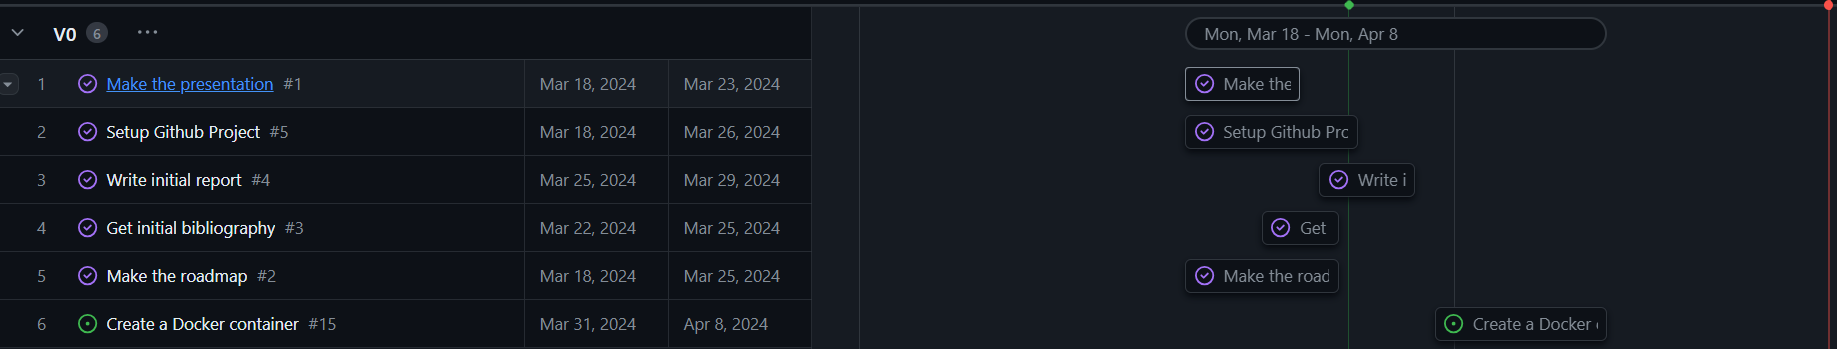
\includegraphics[width=0.7\textwidth]{images/roadmapV0.png}
    \captionsetup{font={scriptsize}}
    \caption{Roadmap for V0}
\end{figure}

\begin{figure}[H]
    \centering
    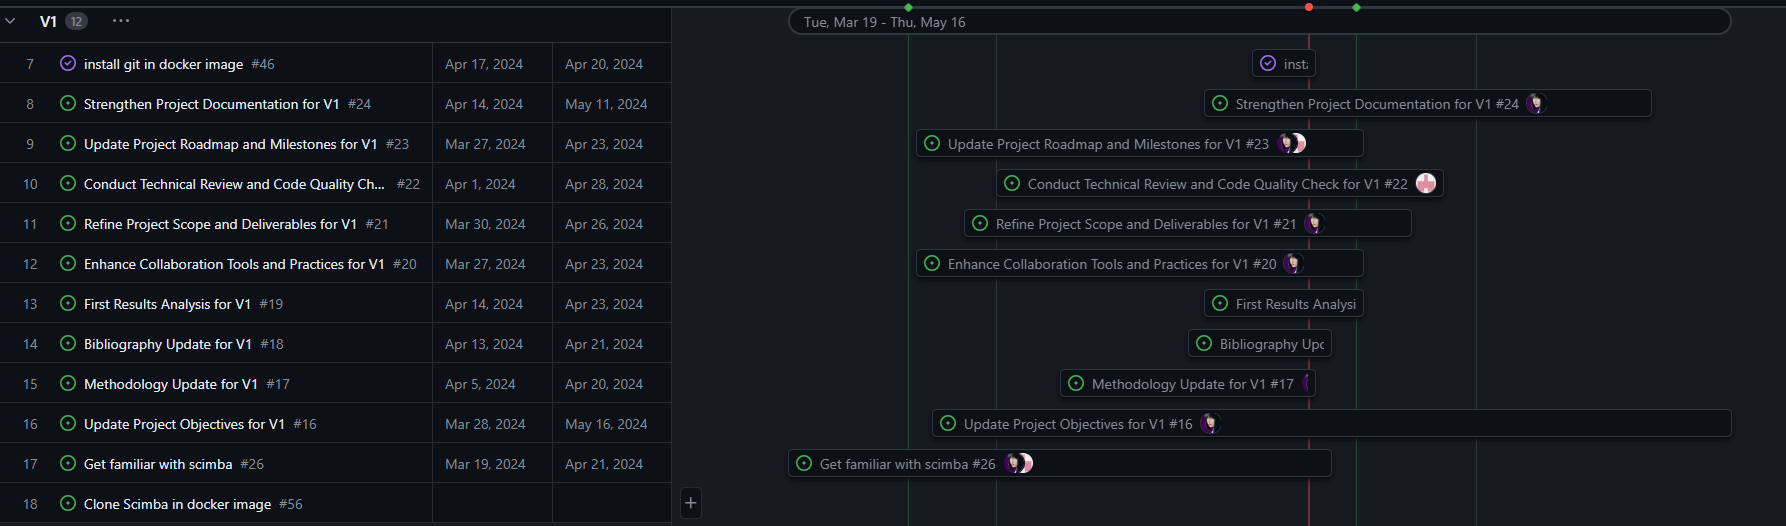
\includegraphics[width=0.7\textwidth]{images/roadmapV1.png}
    \captionsetup{font={scriptsize}}
    \caption{Roadmap for V1}
\end{figure}

\begin{figure}[H]
    \centering
    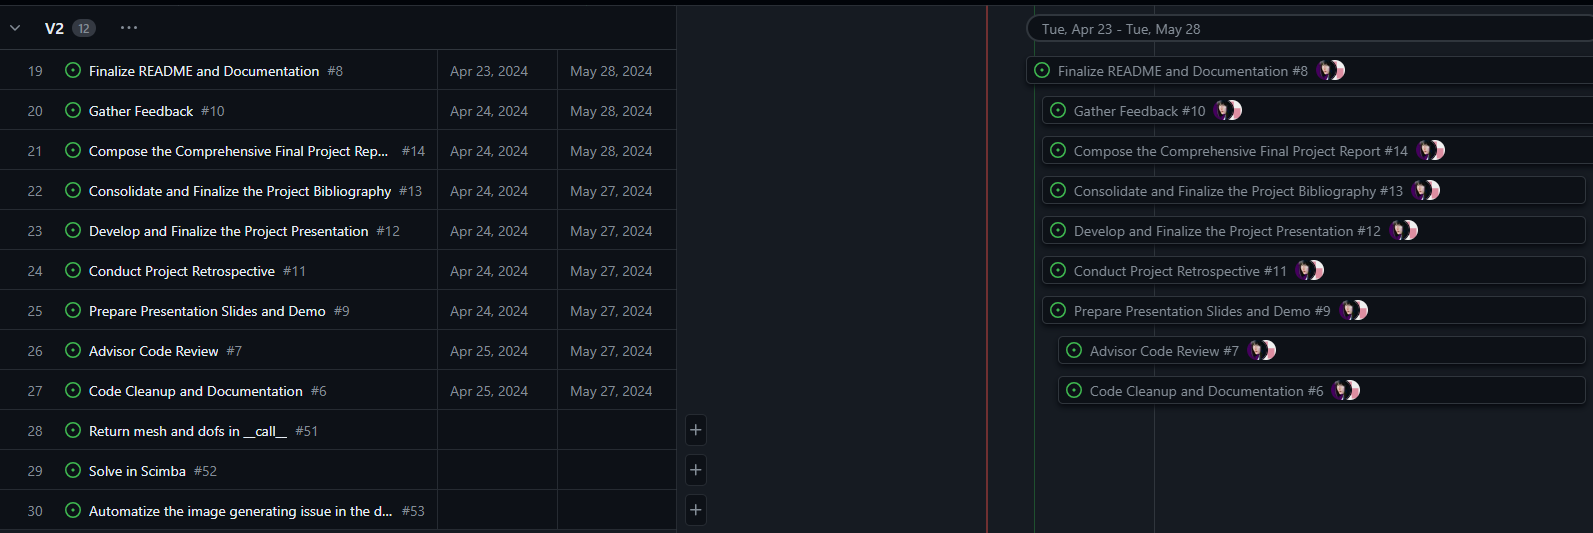
\includegraphics[width=0.7\textwidth]{images/roadmapV2.png}
    \captionsetup{font={scriptsize}}
    \caption{Roadmap for V2}
\end{figure}

%~~~~~~~~~~~~~~~~~~~~~~~~~~~~~~~~~~~~~~~~~~~~~~~~~~~~~~~~~~~~~~
\newpage 

\subsection{Creating a Docker container}
Creating a Docker container and image for the project offers these key advantages:

\begin{enumerate}
    \item \textbf{Portability:} Run the project on any platform supporting Docker.
    \item \textbf{Isolation:} Avoid conflicts with other software on the host system.
    \item \textbf{Reproducibility:} Recreate the exact same environment whenever needed.
    \item \textbf{Dependency Management:} Package all dependencies within the Docker image.
    \\
\end{enumerate}


We're using Feel++ as the base for the Docker container, adding the requirements and dependencies for Scimba and PyTorch.

This Dockerfile contains the latest version of Feel++, Scimba, and PyTorch, and should be able to run these commands without error:
\\
\begin{lstlisting}[language=docker,caption={Dockerfile for Feel++, Scimba, and PyTorch},frame=single, backgroundcolor=\color{gray!10}, basicstyle=\footnotesize,rulecolor=\color{blue}, framexleftmargin=3pt, commentstyle=\color{mygreen}, keywordstyle=\color{blue}]
# Start with the Feel++ base image
FROM ghcr.io/feelpp/feelpp:jammy

# Set labels for metadata
LABEL maintainer="Helya Amiri <helya.amiri@etu.unistra.fr>,
      Rayen Tlili <rayen.tlili@etu.unistra.fr>"
LABEL description="Docker image with Feel++, Scimba, and PyTorch."

# Install PyTorch.
RUN pip3 install torch

# Copy the local Scimba directory to the container.
COPY scimba/ /scimba/

# Install Scimba and its dependencies
WORKDIR /scimba
USER root

RUN pip3 install .

# Set the default command to launch Python.
CMD ["python3"]
\end{lstlisting}


%~~~~~~~~~~~~~~~~~~~~~~~~~~~~~~~~~~~~~~~~~~~~~~~~~~~~~~~~~~~~~~
\newpage


\subsection{Feel++}

Feel++ is a library that allows manipulation of mathematical objects to solve Partial Differential Equations (PDEs). It also provides toolboxes for physics-based models and their coupling. These toolboxes include applications for:

\begin{itemize}
    \item Fluid mechanics
    \item Solid mechanics
    \item Heat transfer and conjugate heat transfer
    \item Fluid-structure interaction
    \item Electro and magnetostatics
    \item Thermoelectrics
    \item Levelset and multifluid
\end{itemize}


\subsection{Exploring Feel++ toolboxes}

As of the first meeting with the project supervisors, we've taken a look at the different toolboxes Feel++ has to offer in Python:
\begin{frame}{}
    \begin{center}
        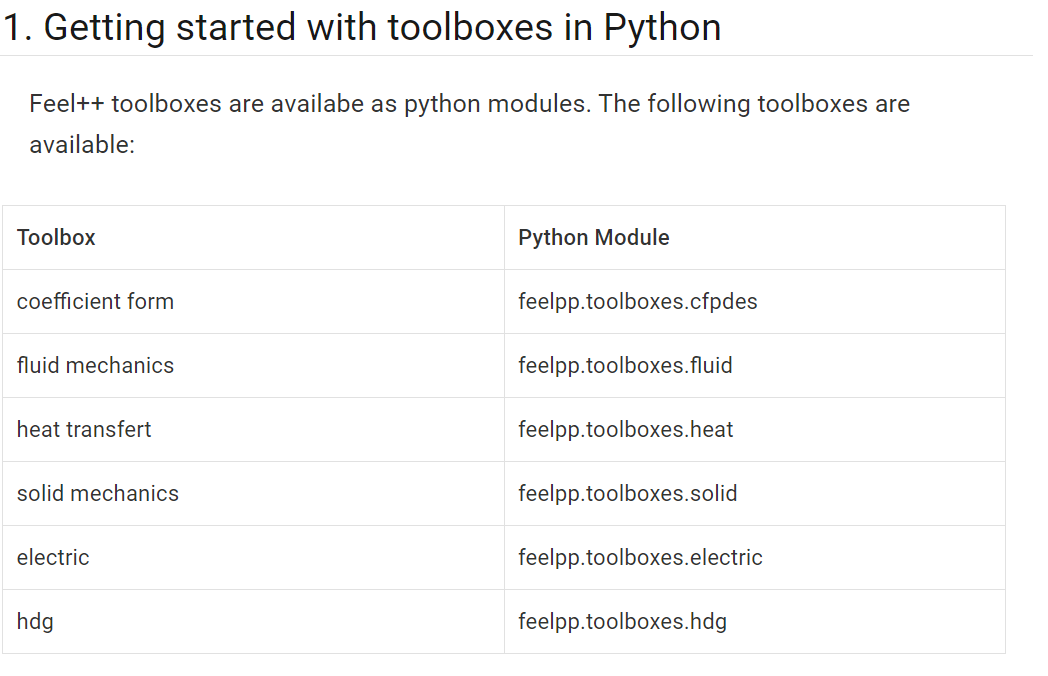
\includegraphics[width=0.7\textwidth]{images/pyfeelpptoolboxes.png}
    \end{center}
\end{frame}

An interesting toolbox to start with is the \textbf{Coefficient Form PDEs}:

%~~~~~~~~~~~~~~~~~~~~~~~~~~~~~~~~~~~~~~~~~~~~~~~~~~~~~~~~~~~~~~
\subsection{Coefficient Form Toolbox}

\begin{enumerate}
    \item \textbf{What are Coefficient Form PDEs?}: The coefficient forms in PDE (Partial Differential Equation) toolboxes encapsulate crucial properties like diffusion, convection, and reaction coefficients. These coefficients are vital for characterizing diverse PDEs such as elliptic, parabolic, or hyperbolic equations, each with its unique coefficient form.
    For instance, in the Poisson equation, a common elliptic equation, the coefficient form is often expressed as:
    \[
        -\nabla \cdot (c \nabla u) + au = f
    \]

    \begin{itemize}
        \item \(c\) : represents the diffusion coefficient,
        \item \(a\) : represents the reaction coefficient,
        \item \(u\) : is the unknown function, and
        \item \(f\) : is the source term.
    \end{itemize}
    
    PDE toolboxes, such as Feel++, offer features for handling different PDEs. They make it easier to define coefficients, set boundaries, discretize problems, and use numerical methods. This helps users to solve complex PDEs, study physical phenomena, and simulate real-world situations more efficiently.

    \item \textbf{System of PDEs}: Many PDEs can be expressed in a standard form, mainly based on the coefficients' definition. We use the following equation to find this form: \\
    \( u \) : \( \Omega \subset \mathbb{R}^d \longrightarrow \mathbb{R}^n \) with \( d = 2, 3 \) and \( n = 1 \) ( \( u \) is a scalar field) or \( n = d \) ( \( u \) is a vector field) such that
    \[
    d \frac{\partial u}{\partial t} + \nabla \cdot \left( -c \nabla u - \alpha u + \gamma \right) + \beta \cdot \nabla u + au = f \text{ in } \Omega
    \]
    \begin{itemize}
        \item \( d \) : damping or mass coefficient
        \item \( c \) : diffusion coefficient
        \item \( \alpha \) : conservative flux convection coefficient
        \item \( \gamma \) : conservative flux source term
        \item \( \beta \) : convection coefficient
        \item \( a \) : absorption or reaction coefficient
        \item \( f \) : source term
    \end{itemize}
    Parameters \( \mu \) may depend on the unknown \( u \) and on the space variable \( x \), time \( t \), and other unknowns \( u_1, \ldots, u_N \).

    \item \textbf{Coefficients}: We also need to follow certain limitations on coefficient shapes, as detailed in the table below.
    \begin{figure}[H]
    \centering
    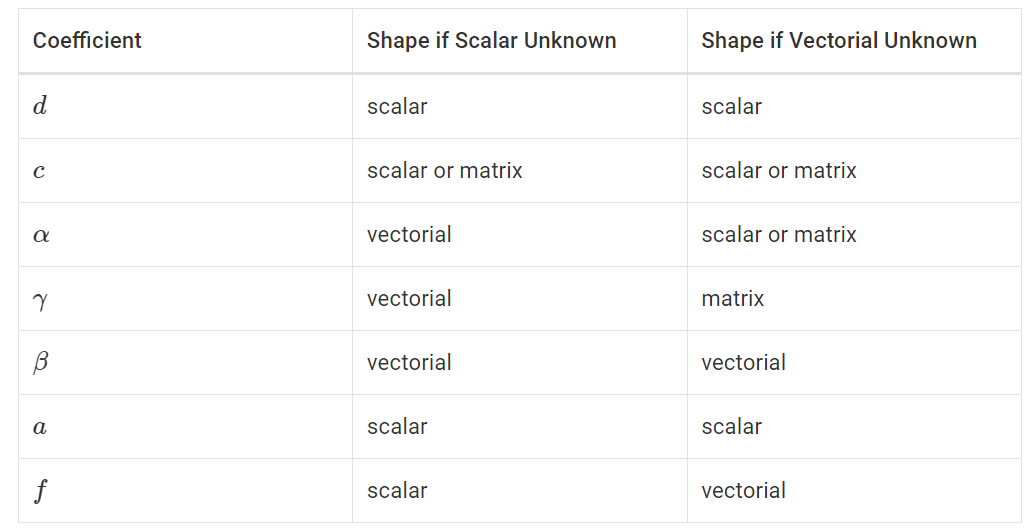
\includegraphics[width=0.7\textwidth]{images/coeff.png}
    \captionsetup{font={scriptsize}}
    \caption{Shape required by the coefficients}
    \end{figure}
    
    \item \textbf{Initial Conditions}: Initial Initial conditions set the initial values for each unknown variable in the equations. These conditions can be defined using expressions or fields.
    
    \textbf{ Boundary Conditions}: 
    \begin{itemize}
        \item Dirichlet
        \item Neumann
        \item Robin
    \end{itemize}
    
    \item \textbf{ Finite Element Approximation}  
    
    \item \textbf{Time scheme}:    
    \begin{itemize}
        \item Backward Differences Formula
        \item Theta scheme
    \end{itemize}  

    \item \textbf{ Stabilized finite element methods}  
    \begin{itemize}
        \item GaLS
        \item SUPG
        \item Coefficient form PDE toolbox        
    \end{itemize} 
 
\end{enumerate}
\end{frame}

%~~~~~~~~~~~~~~~~~~~~~~~~~~~~~~~~~~~~~~~~~~~~~~~~~~~~~~~~~~~~~~
\newpage

\section{Section V1}
\label{sec:Section V1}


%~~~~~~~~~~~~~~~~~~~~~~~~~~~~~~~~~~~~~~~~~~~~~~~~~~~~~~~~~~~~~~
\newpage

\subsection{Objectives for V1}

Once the proper environment was set up in the docker image, we started working on a
program that will solve various PDEs using the Feel++ method and the Scimba method to
visualize and compare the results.


\begin{enumerate}
    \item \textbf{Generate multiple results using Feel++ toolboxes}: Using the CFDE toolbox to solve Poisson equations with varying variables and visualizing them on varying geometries.
    
    \item \textbf{Understanding and exporting results using ScimBa}: Explore the ScimBa repository and use examples from Pinns (Physics-informed neural networks) to solve a simple Poisson equation and visualize the results.
    
    \item \textbf{Creating a program that is able to use both as solvers}: One of the primary objectives to reach for this project is to create a program that is able to call upon the Feel++ CFPDE toolbox and the ScimBa machine learning algorithms to solve various PDEs.
    
    \item \textbf{Comparing the results of both solvers}: The results of both solvers will be able to be visualized and compared in terms of efficiency and accuracy.
\end{enumerate}

After comparing the results of the Poisson equation using both solvers, the work will be working on adapting the program to work on more complex PDEs and other ScimBa neural networks.


\begin{enumerate}
    \setcounter{enumi}{4}
    \item \textbf{Expand Application Scope}: After successfully solving Poisson equations, expand the application of the program to solve other types of PDEs, further demonstrating the versatility of the integrated system.
    
    \item \textbf{Optimize Performance}: Continually optimize the performance of the program, ensuring that it runs efficiently and effectively on various hardware configurations.
    
    \item \textbf{User-Friendly Interface}: Develop a user-friendly interface that allows users with varying levels of technical expertise to utilize the program effectively.
    
    \item \textbf{Documentation and Training}: Provide comprehensive documentation and training materials to help users understand how to use the program and interpret the results.
    
    \item \textbf{Community Engagement}: Engage with the user community to gather feedback, identify areas for improvement, and guide future development efforts.
\end{enumerate}


%~~~~~~~~~~~~~~~~~~~~~~~~~~~~~~~~~~~~~~~~~~~~~~~~~~~~~~~~~~~~~~

\newpage
\subsection{Updating the Docker container}

This Dockerfile creates a docker image with Feel++ as a base and installs the dependencies and libraries needed to run ScimBa in that environment.

It copies the public ScimBa repository into the 'scimba' folder and installs it.

We have also added command lines to automate script that let us run the program 'solvelap.py', that uses Feel++ libraries to solve a Laplacian problem.

\\

\begin{lstlisting}[language=docker,caption={Dockerfile for Feel++, Scimba, and Python libraries.},frame=single, backgroundcolor=\color{gray!10}, basicstyle=\footnotesize,rulecolor=\color{blue}, framexleftmargin=3pt, commentstyle=\color{mygreen}, keywordstyle=\color{blue}]

# Start with the Feel++ base image
FROM ghcr.io/feelpp/feelpp:jammy

# Set labels for metadata
LABEL maintainer="Helya Amiri <helya.amiri@etu.unistra.fr>, 
                  Rayen Tlili <rayen.tlili@etu.unistra.fr>"
LABEL description="Docker image with Feel++, Scimba, and Python libraries."

USER root

# Install system dependencies
RUN apt-get update && apt-get install -y \
    git \
   xvfb

# Install Python libraries
RUN pip3 install torch xvfbwrapper pyvista plotly panel


# Clone the Scimba repository
RUN git clone https://gitlab.inria.fr/scimba/scimba.git /scimba

# Install Scimba and its dependencies
WORKDIR /scimba
RUN pip3 install .

# Copy the xvfb script into the container
COPY tools/load_xvfb.sh /usr/local/bin/load_xvfb.sh
RUN chmod +x /usr/local/bin/load_xvfb.sh

# Set the script to initialize the environment
CMD ["/usr/local/bin/load_xvfb.sh", "python3"]*


\end{lstlisting}



%~~~~~~~~~~~~~~~~~~~~~~~~~~~~~~~~~~~~~~~~~~~~~~~~~~~~~~~~~~~~~~
\newpage
\subsection{Methodology}
Given the Feel++ documentation and the Poisson class prototype that gives access to results from the Feel++ solver.

Create the right environment for using the CFPDE toolbox:
\begin{lstlisting}[language=python,caption={},frame=single, backgroundcolor=\color{gray!10}, basicstyle=\footnotesize,rulecolor=\color{blue}, framexleftmargin=3pt, commentstyle=\color{mygreen}, keywordstyle=\color{blue}]

import sys
import feelpp
import feelpp.toolboxes.core as tb

from tools.solvers import Poisso
sys.argv = ["feelpp_app"]
e = feelpp.Environment(sys.argv,
                       opts=tb.toolboxes_options("coefficient-form-pdes", 
                       "cfpdes"),
                       config=feelpp.globalRepository('feelpp_cfpde'))

\end{lstlisting}

Solving the Poisson equation with different parameters using the CFPDE toolbox

\begin{lstlisting}[language=Python,caption={},frame=single, backgroundcolor=\color{gray!10}, basicstyle=\footnotesize,rulecolor=\color{blue}, framexleftmargin=3pt, commentstyle=\color{mygreen}, keywordstyle=\color{blue}]

P = Poisson(dim = 2)
P(h=0.08,  rhs='-1.0-1*y*x+y*y', g='0', order=1, geofile='geo/disk.geo',
    plot='2d.png')
P(h=0.1,  rhs='-1.0-2*y*x+y*y', g='0', order=1, plot='f2.png')

P = Poisson(dim = 2)
P(h=0.1, diff='{1.0,0,0,x*y}', rhs='1', plot='d1.png')
P(h=0.1, diff='{1+x,0,0,1+y}', rhs='1', plot='d2.png')

P = Poisson(dim = 3)
P(h=0.08, diff='{1,0,0,0,x+1,0,0,0,1+x*y}', g = 'x', rhs='x*y*z', 
geofile = 'geo/cube.geo', plot='3d.png') 

\end{lstlisting}

Adding the option to use a different solver when calling the Poisson Class.
\begin{lstlisting}[language=Python,caption={},frame=single, backgroundcolor=\color{gray!10}, basicstyle=\footnotesize,rulecolor=\color{blue}, framexleftmargin=3pt, commentstyle=\color{mygreen}, keywordstyle=\color{blue}]
def __call__(self,
               h,                                       # mesh size 
               order=1,                                 # polynomial order 
               name='Potential',                        # name of the variable
               rhs='8*pi*pi*sin(2*pi*x)*sin(2*pi*y)',   # right hand side
               diff='{1,0,0,1}',                        # diffusion matrix
               g='0',
               geofile=None,
               plot=None,
               solver='feelpp'):                        # or solver ='scimba'
    """
\end{lstlisting}

%~~~~~~~~~~~~~~~~~~~~~~~~~~~~~~~~~~~~~~~~~~~~~~~~~~~~~~~~~~~~~~
\newpage

Solve using feelpp tools and a space to return the same types of results using ScimBa

\begin{lstlisting}[language=Python,caption={},frame=single, backgroundcolor=\color{gray!10}, basicstyle=\footnotesize,rulecolor=\color{blue}, framexleftmargin=3pt, commentstyle=\color{mygreen}, keywordstyle=\color{blue}]

if solver == 'feelpp':
      print(f"Solving the laplacian problem for hsize = {h}...")
      feelpp_mesh = feelpp.load(feelpp.mesh(dim=self.dim, realdim=self.dim), 
                                fn, h)
      self.pb.setMesh(feelpp_mesh)
      self.pb.setModelProperties(self.model)
      self.pb.init(buildModelAlgebraicFactory=True)
      self.pb.printAndSaveInfo()
      self.pb.solve()
      self.pb.exportResults()
    
      #measures = self.pb.postProcessMeasures().values()

elif solver == 'scimba':
     print("Solving using Scimba")
     # the solution process using Scimba
      return
      
\end{lstlisting}

We would wanna use this do generate results exctracted from ScimBa:

\begin{lstlisting}[language=Python,caption={},frame=single, backgroundcolor=\color{gray!10}, basicstyle=\footnotesize,rulecolor=\color{blue}, framexleftmargin=3pt, commentstyle=\color{mygreen}, keywordstyle=\color{blue}]

P(h=0.08, diff='{1,0,0,0,x+1,0,0,0,1+x*y}', g = 'x', rhs='x*y*z', geofile = 
'geo/cube.geo', plot='3d.png', solver='scimba') 

\end{lstlisting}

%~~~~~~~~~~~~~~~~~~~~~~~~~~~~~~~~~~~~~~~~~~~~~~~~~~~~~~~~~~~~~~
\newpage

\subsection{Getting familiar with ScimBa}

We decided to start using the examples in the ScimBa repository of uses of the Physics-Informed Neural Networks (PINNs). PINNs integrate the underlying physical laws described by PDEs directly into the learning process of neural networks. This is achieved by constructing a loss function that penalizes the network for failing to fit known data and for violating the given physical laws.

\begin{lstlisting}[language=Python,caption={},frame=single, backgroundcolor=\color{gray!10}, basicstyle=\footnotesize,rulecolor=\color{blue}, framexleftmargin=3pt, commentstyle=\color{mygreen}, keywordstyle=\color{blue}]

from lap2D_pinns import Run_laplacian2D, Poisson_2D
from scimba.equations import domain


# Define a square domain
xdomain = domain.SpaceDomain(2, domain.SquareDomain(2, [[0.0, 1.0], 
                                                    [0.0, 1.0]]))

# Create an instance of the Poisson problem
pde = Poisson_2D(xdomain)

# Run the training
Run_laplacian2D(pde)

\end{lstlisting}

The class Poisson 2D is initialized with a given spatial domain (space domain) and sets up the problem with one unknown variable and one parameter.
The parameter domain is narrowly defined, likely to enforce precise boundary conditions or to stabilize the solution.
\begin{lstlisting}[language=Python,caption={},frame=single, backgroundcolor=\color{gray!10}, basicstyle=\footnotesize,rulecolor=\color{blue}, framexleftmargin=3pt, commentstyle=\color{mygreen}, keywordstyle=\color{blue}]
class Poisson_2D(pdes.AbstractPDEx):
    def __init__(self, space_domain):
        super().__init__(
            nb_unknowns=1,
            space_domain=space_domain,
            nb_parameters=1,
            parameter_domain=[[0.50000, 0.500001]],
        )

\end{lstlisting}


The Run laplacian2D function encapsulates the entire process of setting up, training, and evaluating a neural network to solve the Laplacian PDE using PINN. This includes data sampling, network configuration, loss calculation, and optimization.

\begin{lstlisting}[language=Python,caption={},frame=single, backgroundcolor=\color{gray!10}, basicstyle=\footnotesize,rulecolor=\color{blue}, framexleftmargin=3pt, commentstyle=\color{mygreen}, keywordstyle=\color{blue}]

def Run_laplacian2D(pde, bc_loss_bool=False, w_bc=0, w_res=1.0):
    x_sampler = sampling_pde.XSampler(pde=pde)
    mu_sampler = sampling_parameters.MuSampler(
        sampler=uniform_sampling.UniformSampling, model=pde
    )
    sampler = sampling_pde.PdeXCartesianSampler(x_sampler, mu_sampler)

\end{lstlisting}
%~~~~~~~~~~~~~~~~~~~~~~~~~~~~~~~~~~~~~~~~~~~~~~~~~~~~~~~~~~~~~~
\newpage
If new training = False, the code suggests that you might want to continue using a previously trained and saved model without starting the training from scratch.
If new training = True, it indicates that you want to start fresh, ignoring any previously saved models.
\begin{lstlisting}[language=Python,caption={},frame=single, backgroundcolor=\color{gray!10}, basicstyle=\footnotesize,rulecolor=\color{blue}, framexleftmargin=3pt, commentstyle=\color{mygreen}, keywordstyle=\color{blue}]

    new_training = False
    #new_training = True
    if new_training:
        (
            Path.cwd()
            / Path(training_x.TrainerPINNSpace.FOLDER_FOR_SAVED_NETWORKS)
            / file_name
        ).unlink(missing_ok=True)
        
\end{lstlisting}

We will talk further about the files and visuals generated in both cases in the "Results" section.
\\
Other neural networks available on ScimBa:
\begin{frame}{}
    \begin{center}
        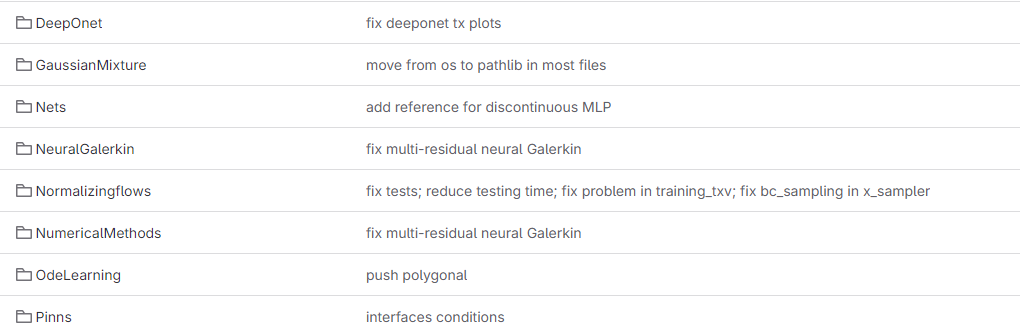
\includegraphics[width=0.7\textwidth]{images/ScimBa neural networks.png}
    \end{center}
\end{frame}

%~~~~~~~~~~~~~~~~~~~~~~~~~~~~~~~~~~~~~~~~~~~~~~~~~~~~~~~~~~~~~~


\newpage

\section{Section V2}
\label{sec:Section V2}

%~~~~~~~~~~~~~~~~~~~~~~~~~~~~~~~~~~~~~~~~~~~~~~~~~~~~~~~~~~~~~~
\newpage

\subsection{Future Work}

The next phase of our project, referred to as V2, has several open issues that need to be addressed:

\begin{itemize}
    \item Automatize the image generating issue in the docker (\href{https://github.com/master-csmi/2024-m1-scimba-feelpp/issues/52}{Issue \#52})
    \item Solve in ScimBa (\href{https://github.com/master-csmi/2024-m1-scimba-feelpp/issues/51}{Issue \#51})
    \item Return mesh and dofs in \_\_call\_\_ (\href{https://github.com/master-csmi/2024-m1-scimba-feelpp/issues/6}{Issue \#6})
    \item Code Cleanup and Documentation (\href{https://github.com/master-csmi/2024-m1-scimba-feelpp/issues/7}{Issue \#7})
    \item Advisor Code Review (\href{https://github.com/master-csmi/2024-m1-scimba-feelpp/issues/9}{Issue \#9})
    \item Prepare Presentation Slides and Demo (\href{https://github.com/master-csmi/2024-m1-scimba-feelpp/issues/11}{Issue \#11})
    \item Conduct Project Retrospective (\href{https://github.com/master-csmi/2024-m1-scimba-feelpp/issues/12}{Issue \#12})
    \item Develop and Finalize the Project Presentation (\href{https://github.com/master-csmi/2024-m1-scimba-feelpp/issues/13}{Issue \#13})
    \item Consolidate and Finalize the Project Bibliography (\href{https://github.com/master-csmi/2024-m1-scimba-feelpp/issues/14}{Issue \#14})
    \item Compose the Comprehensive Final Project Report (\href{https://github.com/master-csmi/2024-m1-scimba-feelpp/issues/10}{Issue \#10})
    \item Gather Feedback (\href{https://github.com/master-csmi/2024-m1-scimba-feelpp/issues/8}{Issue \#8})
    \item Finalize README and Documentation (\href{https://github.com/master-csmi/2024-m1-scimba-feelpp/issues/8}{Issue \#8})
\end{itemize}

These issues represent the key tasks that will be undertaken in the V2 phase of the project. Each issue is linked to its corresponding GitHub issue for easy tracking and reference.

%~~~~~~~~~~~~~~~~~~~~~~~~~~~~~~~~~~~~~~~~~~~~~~~~~~~~~~~~~~~~~~
\newpage

\section{Results}
\subsection{Generating visuals using Feel++}

Using the Poisson class and the Laplacian2D.py program,


\begin{lstlisting}[language=Python,caption={},frame=single, backgroundcolor=\color{gray!10}, basicstyle=\footnotesize,rulecolor=\color{blue}, framexleftmargin=3pt, commentstyle=\color{mygreen}, keywordstyle=\color{blue}]
def genCube(self, filename, h=0.1):
    """
    Generate a cube geometry following the dimension  self.dim
    """

    
    geo="""SetFactory("OpenCASCADE");
    h={};
    dim={};
    """.format(h, self.dim)
    
    if self.dim==2 :
        geo+="""
        Rectangle(1) = {0, 0, 0, 1, 1, 0};
        Characteristic Length{ PointsOf{ Surface{1}; } } = h;
        Physical Curve("Gamma_D") = {1,2,3,4};
        Physical Surface("Omega") = {1};
        """
    elif self.dim==3 :
        geo+="""
        Box(1) = {0, 0, 0, 1, 1, 1};
        Characteristic Length{ PointsOf{ Volume{1}; } } = h;
        Physical Surface("Gamma_D") = {1,2,3,4,5,6};
        Physical Volume("Omega") = {1};
        """
    with open(filename, 'w') as f:
        f.write(geo
\end{lstlisting}

Generated 3D geometry and mesh viewed using gmsh:

\begin{frame}{}
        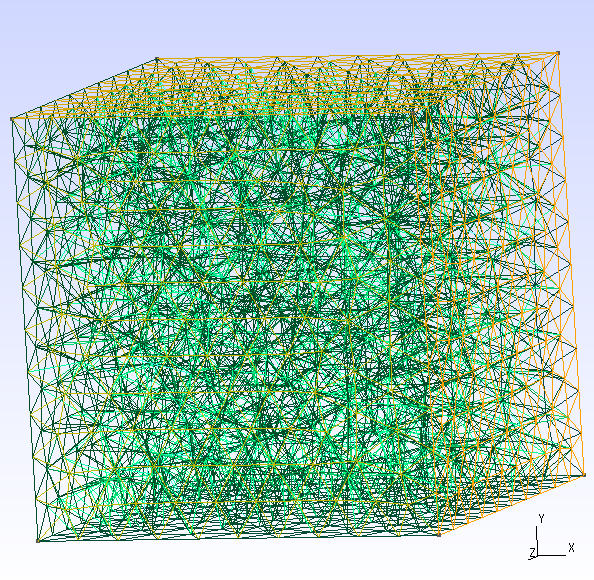
\includegraphics[width=0.4\textwidth]{images/fppmsh.png}
\end{frame}


Viewing 3D and 2D plotting viewed using paraview:

\begin{frame}{}
    \begin{center}
        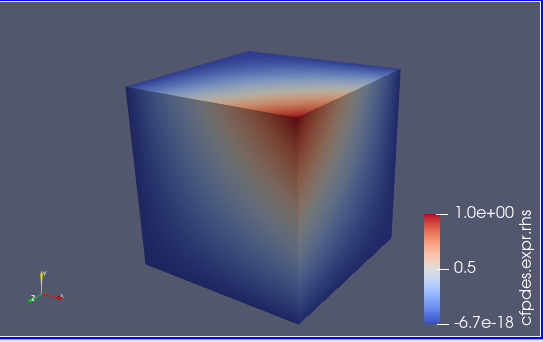
\includegraphics[width=0.7\textwidth]{images/paraview 3d.png}
        \includegraphics[width=0.7\textwidth]{images/laplacian2d2d.png}
    \end{center}
\end{frame}

%~~~~~~~~~~~~~~~~~~~~~~~~~~~~~~~~~~~~~~~~~~~~~~~~~~~~~~~~~~~~~~
\newpage

\subsection{Generating visuals using ScimBa}
\begin{lstlisting}[language=Python,caption={},frame=single, backgroundcolor=\color{gray!10}, basicstyle=\footnotesize,rulecolor=\color{blue}, framexleftmargin=3pt, commentstyle=\color{mygreen}, keywordstyle=\color{blue}]
    xdomain = domain.SpaceDomain(2, domain.SquareDomain(2, [[0.0, 1.0], 
                                                        [0.0, 1.0]]))
    print(xdomain)
    pde = Poisson_2D(xdomain)
    Run_laplacian2D(pde)
    
\end{lstlisting}
    
Laplacian strong Bc on Square with nn
\begin{frame}{}
    \begin{center}
        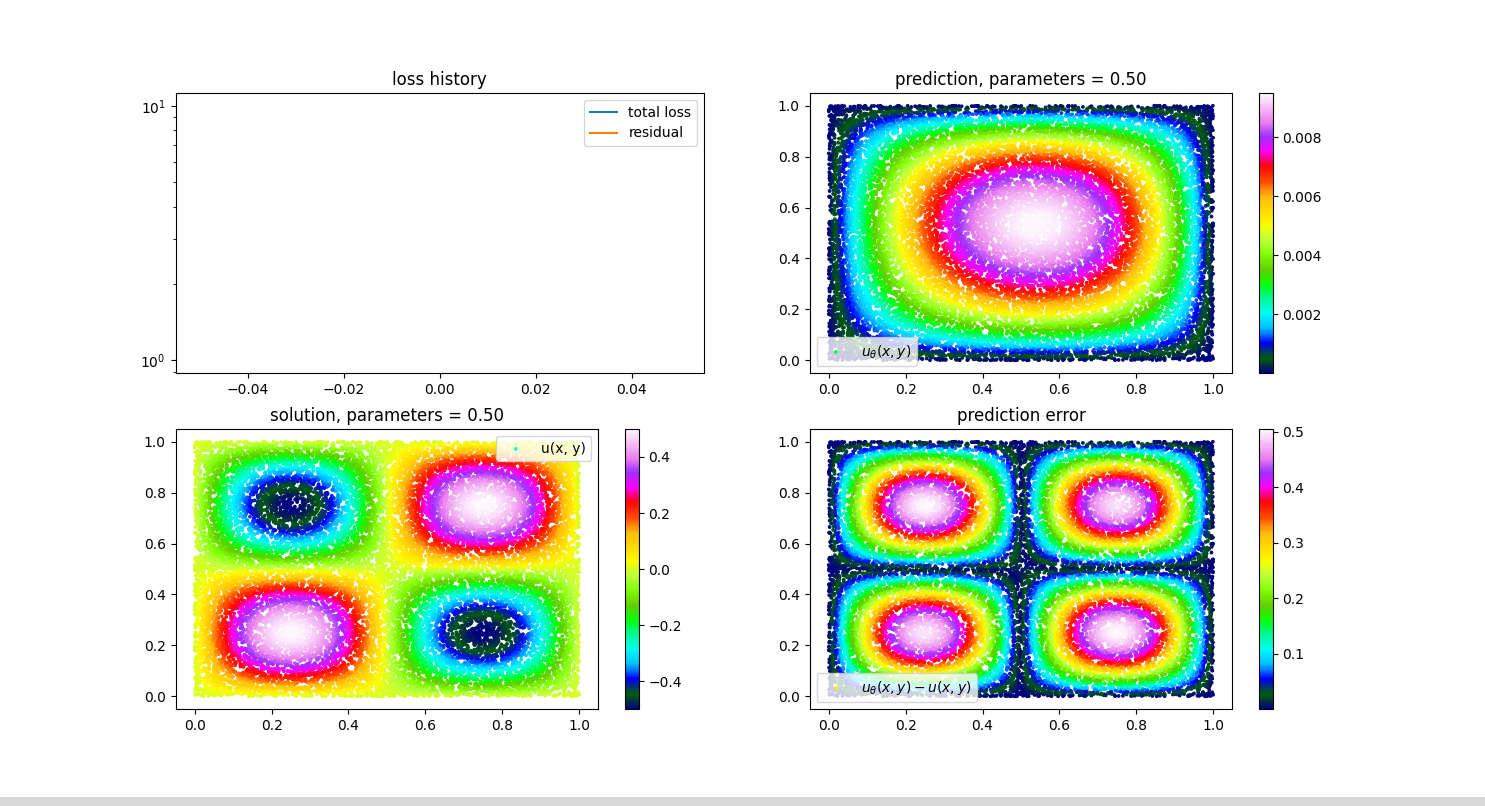
\includegraphics[width=0.7\textwidth]{images/scimbaplot1.png}
    \end{center}
\end{frame}
Laplacian on circle with nn
\begin{lstlisting}[language=Python,caption={},frame=single, backgroundcolor=\color{gray!10}, basicstyle=\footnotesize,rulecolor=\color{blue}, framexleftmargin=3pt, commentstyle=\color{mygreen}, keywordstyle=\color{blue}]
    xdomain = domain.SpaceDomain(2, domain.DiskBasedDomain(2, [0.5, 0.5], 1.0))
    pde = PoissonDisk2D(xdomain)
    Run_laplacian2D(pde, bc_loss_bool=True, w_bc=10, w_res=0.1)
    
\end{lstlisting}
\begin{frame}{}
    \begin{center}
        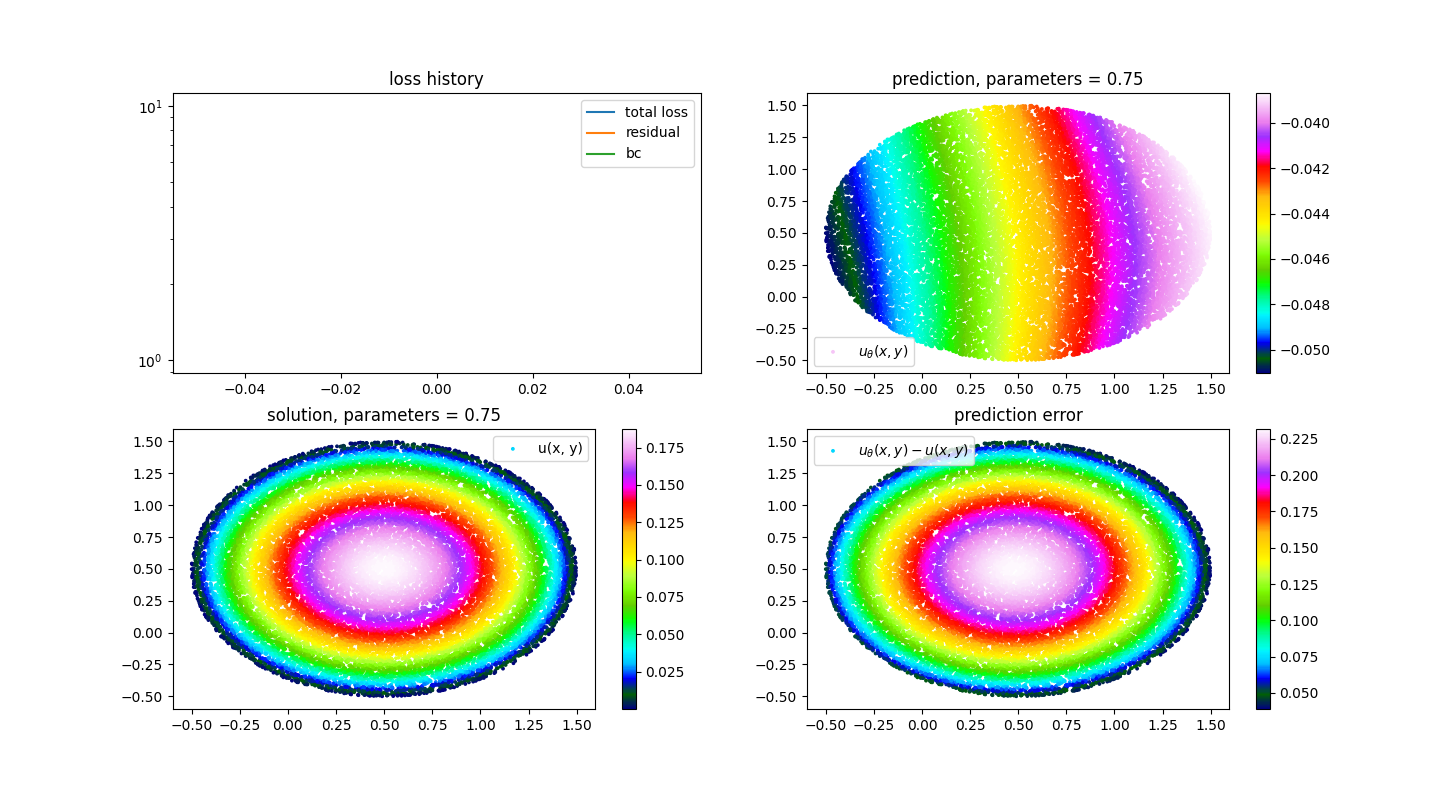
\includegraphics[width=0.7\textwidth]{images/scimbaplot2.png}
        \end{center}
\end{frame}

%~~~~~~~~~~~~~~~~~~~~~~~~~~~~~~~~~~~~~~~~~~~~~~~~~~~~~~~~~~~~~~
\newpage

Laplacian on ellipse and mapping with nn
\begin{lstlisting}[language=Python,caption={},frame=single, backgroundcolor=\color{gray!10}, basicstyle=\footnotesize,rulecolor=\color{blue}, framexleftmargin=3pt, commentstyle=\color{mygreen}, keywordstyle=\color{blue}]
    xdomain = domain.SpaceDomain(
        2,
        domain.DiskBasedDomain(
            2,
            [0.0, 0.0],
            1.0,
            mapping=disk_to_ellipse,
            Jacobian=Jacobian_disk_to_ellipse,
        ),
    )
    pde = Poisson_2D_ellipse(xdomain)
    Run_laplacian2D(pde, bc_loss_bool=True, w_bc=10, w_res=0.1)
    
\end{lstlisting}
\begin{frame}{}
    \begin{center}
        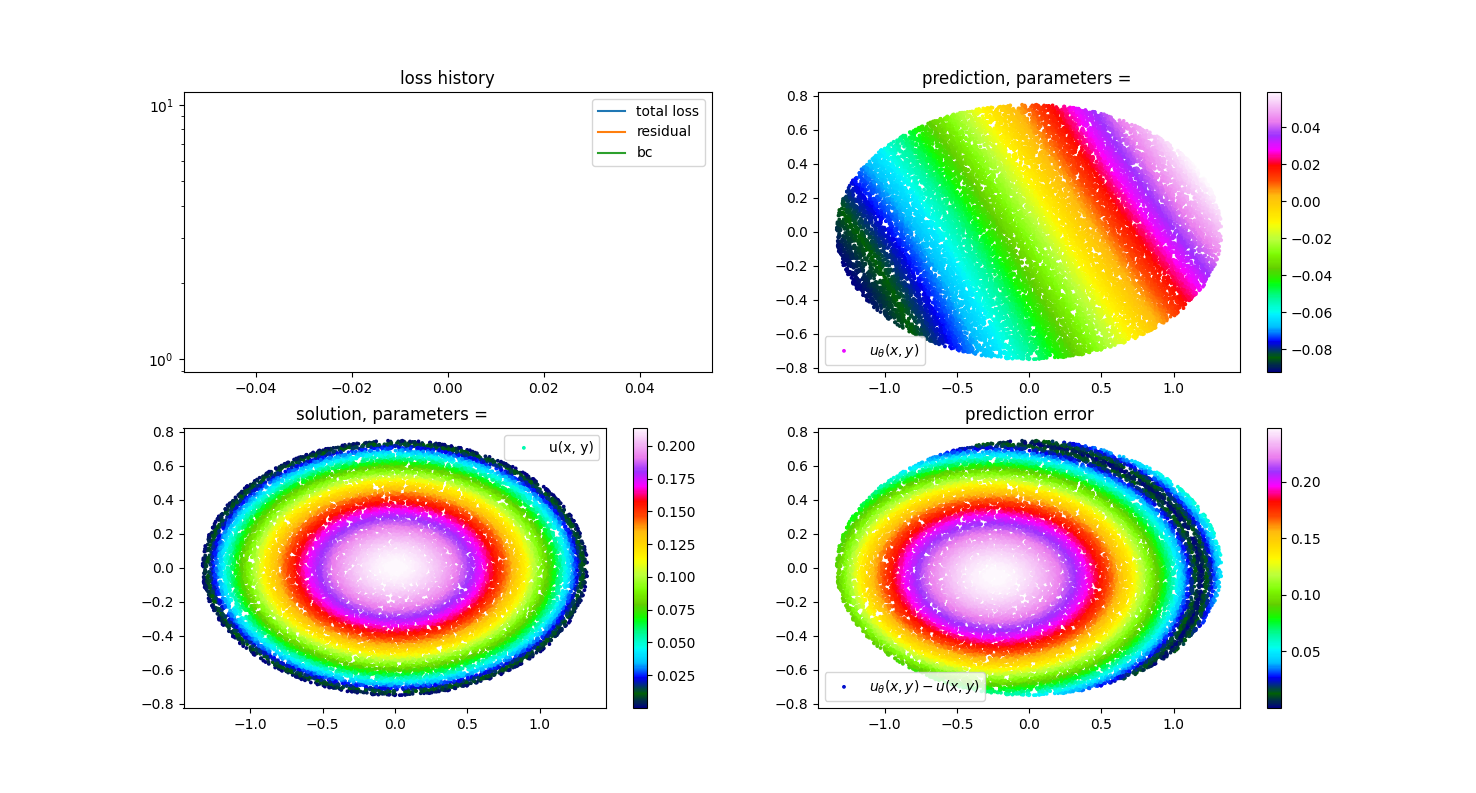
\includegraphics[width=0.7\textwidth]{images/scimbaplot3.png}
        \end{center}
\end{frame}
Laplacian on potato and mapping with nn
\begin{lstlisting}[language=Python,caption={},frame=single, backgroundcolor=\color{gray!10}, basicstyle=\footnotesize,rulecolor=\color{blue}, framexleftmargin=3pt, commentstyle=\color{mygreen}, keywordstyle=\color{blue}]
    xdomain = domain.SpaceDomain(2, domain.SquareDomain(2, [[0.0, 1.0], 
                                                        [0.0, 1.0]]))
    print(xdomain)
    pde = Poisson_2D(xdomain)
    Run_laplacian2D(pde)
    
\end{lstlisting}
\begin{frame}{}
    \begin{center}
        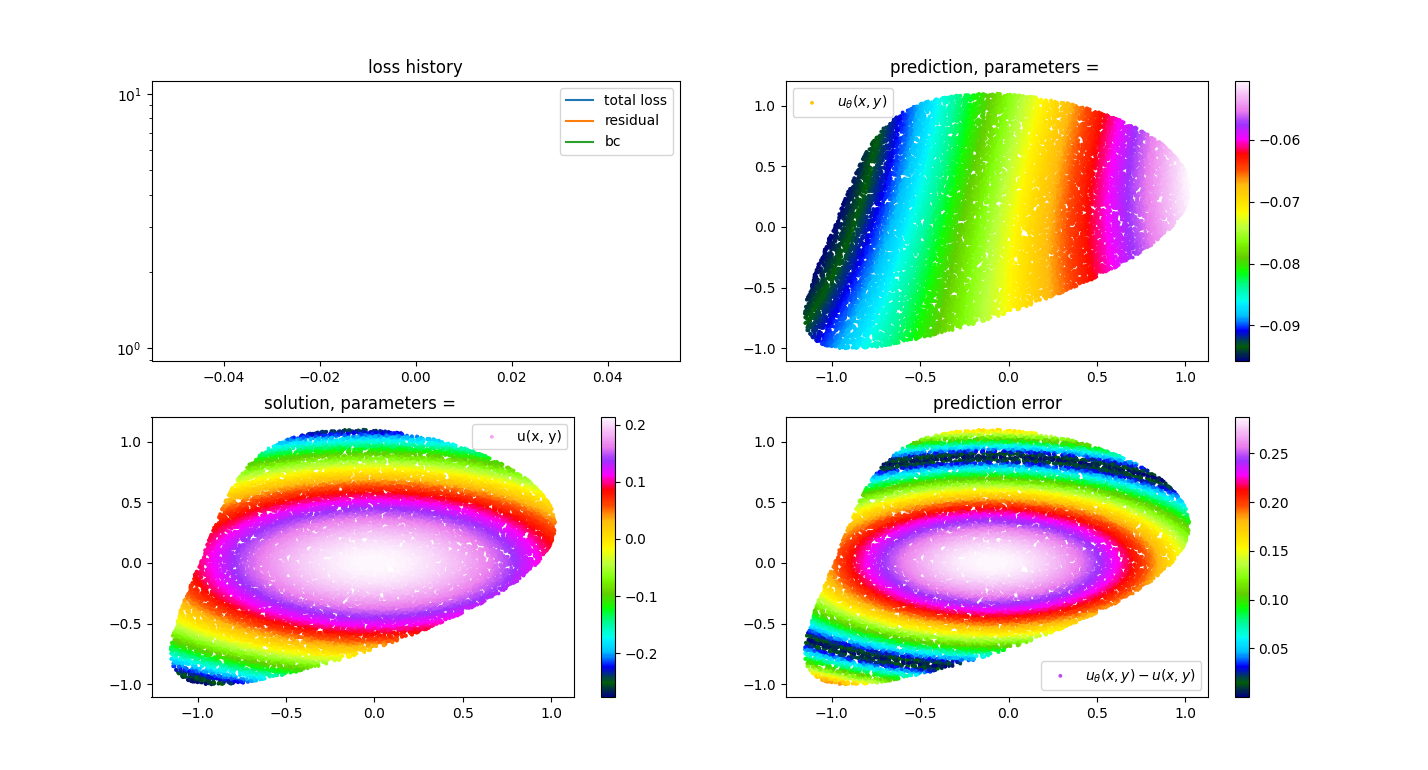
\includegraphics[width=0.7\textwidth]{images/scimbaplot4.png}

    \end{center}
\end{frame}


%~~~~~~~~~~~~~~~~~~~~~~~~~~~~~~~~~~~~~~~~~~~~~~~~~~~~~~~~~~~~~~
\newpage

\section{Conclusion}

%~~~~~~~~~~~~~~~~~~~~~~~~~~~~~~~~~~~~~~~~~~~~~~~~~~~~~~~~~~~~~~
\newpage

\part*{Bibliography}
\addcontentsline{toc}{part}{\textit{Bibliography}}
\bibliographystyle{unsrt}
\bibliography{References.bib}

\begin{thebibliography}{14}

\bibitem{feelpp}
Feel++. (n.d.). \textit{Modeling and Quantitative Simulation}. Retrieved from \url{https://feelpp.github.io/mqs/cases/0.109/index.html}

\bibitem{pyfeelpptoolboxes}
Feel++. (n.d.). \textit{Python Feel++ Toolboxes}. Retrieved from \url{https://docs.feelpp.org/user/latest/python/pyfeelpptoolboxes/index.html}

\bibitem{mso4sc}
MSO4SC. (n.d.). \textit{Poisson}. Retrieved from \url{https://book.mso4sc.cemosis.fr/cases/0.109/poisson/README/}

\bibitem{zenodo}
Zenodo. (n.d.). \textit{Zenodo Record}. Retrieved from \url{https://zenodo.org/records/1231527}


\bibitem{sciml}
SciML. (n.d.). \textit{Laplacian 2D Disk}. Retrieved from \url{https://sciml.gitlabpages.inria.fr/scimba/examples/laplacian2DDisk.html}

\bibitem{scimba}
ScimBa. (n.d.). \textit{ScimBa Repository}. Retrieved from \url{https://gitlab.inria.fr/scimba/scimba}

\bibitem{feelppgithub}
Feel++. (n.d.). \textit{Feel++ GitHub Repository}. Retrieved from \url{https://github.com/feelpp/feelpp}

\bibitem{cemosis}
Cemosis. (n.d.). \textit{Course: Solving PDEs with Feel++}. Retrieved from \url{https://www.cemosis.fr/events/course-solving-pdes-with-feel/}

\bibitem{mso4scbook}
MSO4SC. (n.d.). \textit{Feel++ Book}. Retrieved from \url{https://book.mso4sc.cemosis.fr/feelpp/}

\bibitem{coupling}
Wikipedia. (n.d.). \textit{Coupling (computer programming)}. Retrieved from \url{https://en.wikipedia.org/wiki/Coupling_(computer_programming)}

\bibitem{scimba2}
SciML. (n.d.). \textit{ScimBa}. Retrieved from \url{https://sciml.gitlabpages.inria.fr/scimba/}

\bibitem{feelppdocs}
Feel++. (n.d.). \textit{Feel++ Documentation}. Retrieved from \url{https://docs.feelpp.org/user/latest/index.html}

\bibitem{Quick Start with Docker}
Feel++. (n.d.). \textit{Quick Start with Docker}. Retrieved from \url{https://docs.feelpp.org/user/latest/using/docker.html}

\bibitem{Mixed Poisson}
Feel++. (n.d.). \textit{Mixed Poisson}. Retrieved from \url{https://docs.feelpp.org/user/latest/using/toolboxes/hdg_poisson.html}

\end{thebibliography}




\end{document}

%Fin :)